%%---------------------------------------------------------------------------%%
%% req_doc_7_1999.tex
%% John Gulick
%% Time-stamp: <99/07/23 10:52:55 gulick>
%%---------------------------------------------------------------------------%%
\documentclass[11pt]{nmemo}
\usepackage[centertags]{amsmath}
\usepackage{amssymb,amsthm,graphicx}
\usepackage[mathcal]{euscript}
\usepackage{tmadd,tmath}
\usepackage{cite}

%%---------------------------------------------------------------------------%%
%% DEFINE SPECIFIC ENVIRONMENTS HERE
%%---------------------------------------------------------------------------%%
%\newcommand{\elfit}{\ensuremath{\operatorname{Im}(-1/\epsilon(\vq,\omega)}}
%\msection{}-->section commands
%\tradem{}  -->add TM subscript to entry
%\ucatm{}   -->add trademark footnote about entry

%%---------------------------------------------------------------------------%%
%% BEGIN DOCUMENT
%%---------------------------------------------------------------------------%%
\begin{document}

%%---------------------------------------------------------------------------%%
%% OPTIONS FOR NOTE
%%---------------------------------------------------------------------------%%

\toms{Todd Urbatsch, Tom Evans, Todd Wareing/XTM MS D409}
%\toms{Joe Sixpak/XTM, MS B226}
\refno{XTM:99-51(U)}
\subject{DRACO Fourier Analysis Package: Requirements Document}

%-------NO CHANGES
\divisionname{Applied Theoretical \& Computational Physics Div.}
\groupname{X-TM:Transport Methods Group}
\fromms{John C. Gulick/XTM D409}
\phone{(505)667--5790}
\originator{gulick}
\typist{gulick}
\date{July 23, 1999}
%-------NO CHANGES

%-------OPTIONS
%\reference{NPB Star Reimbursable Project}
%\thru{P. D. Soran, XTM, MS B226}
%\enc{list}      
%\attachments{list}
%\cy{list}
%\encas
%\attachmentas
%\attachmentsas 
%-------OPTIONS

%%---------------------------------------------------------------------------%%
%% DISTRIBUTION LIST
%%---------------------------------------------------------------------------%%
\distribution {}
%%---------------------------------------------------------------------------%%
%% BEGIN NOTE
%%---------------------------------------------------------------------------%%

\opening
\section{Introduction}
As part of the continuing development of the Draco
radiation-transport oriented software-engineering system, a Fourier
analysis package is being designed to further extend the capabilities
of the system.  This piece of software is being written
so as to conform to the fundamentals of Design by 
Contract$^{\tt TM}$\footnote{``Design by Contract'' is a 
trademark of Interactive Software Engineering.} (DBC)~\cite{me97}. This 
document lists the requirements of the Fourier analysis package, and it
provides a guide for its development by defining the project's scope.
\section{Project Requirements}
The requirements of the Fourier analysis package project fall into
three categories:
\begin{description}
 \item [Technical Requirements] Requirements having to do with the
   Fourier analysis capability, specifications and scope of the project.
 \item [Software Requirements] Requirements having to do with the
   programming/coding aspects of the Fourier analysis package.
 \item [Testing Requirements] Requirements having to do with the
 testing and verification of the Fourier analysis package.
\end{description}
\subsection{Technical Requirements}
\begin{enumerate}
 \item The purpose of this project is to provide one- and
   two-dimensional Fourier analysis
   capability for deterministic radiation transport discretizations. 
 \item Analyses for:
 \begin{itemize}
  \item $\rho$ vs. $\Delta_x$, $\Delta_y$ (Any range with
    user-selectable resolution and any subsequent refinement)
  \item $\rho$ vs. $\lambda_x$, $\lambda_y$ (User selectable range,
    usually from 0 to $\pi$)
  \item $\rho$ vs. Aspect Ratio ($\Delta_x$/$\Delta_y$)
 \end{itemize}
 \item Allow user to create two- and three-dimensional plots of the
   Fourier analysis results.
 \item User-supplied Fourier matrix generation routine: 
 \begin{itemize}
  \item Calculates Fourier matrix for each desired set of input
    conditions.  These conditions would include varying cross sections, 
    $\sigma_{t,s,a}$, varying cell thicknesses,
    $\Delta_{x,y}$, varying ranges of optical thicknesses
    (number of mean-free-paths), and so on.
  \item This matrix may include an acceleration operator such as DSA, TSA, or
    multi-grid, the form of which the user would supply. 
 \end{itemize}
 \item Requires multiple complex linear algebra routines:
 \begin{itemize}
  \item Requires a complex ${N \times N}$ matrix inversion routine.
  \item Requires a complex ${N \times N}$ matrix multiplication routine.
  \item Requires a robust complex ${N \times N}$ eigenvalue/eigenvector solver.
 \end{itemize}
 \item Requires a quadrature set capable of multi-dimensional
   integration.  The most promising appears to be a
   Chebyshev-Legendre quadrature set developed by Wallace Walters.
   Other types of quadratures, for different types of problems, could
   be included as well with little difficulty. 
\end{enumerate}
\subsection{Software Requirements}
\begin{enumerate}
 \item The package will consist of four main components:
 \begin{itemize}
  \item ${Preprocessor}$ Component
  \item ${Fourier\_Matrix}$ Component
  \item ${LinAlg}$ Component
  \item ${Postprocessor}$ Component
 \end{itemize}
 \item This is a flow diagram of the components and their major
   responsibilities.
 \begin{figure}[htbp]
  \begin{centering}
   \begin{center}
    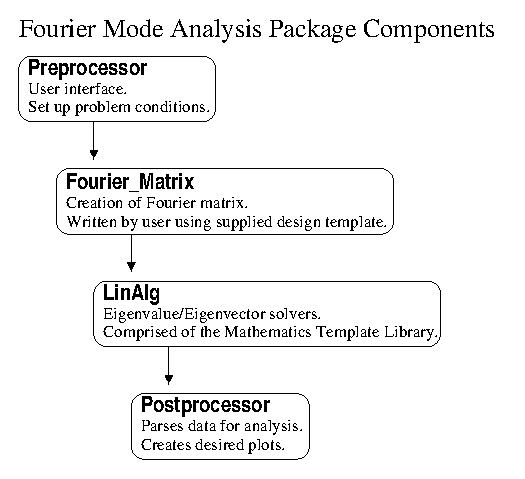
\includegraphics[scale=1.0]{components.eps}
   \end{center}
   \caption{Flow diagram of components and their major responsibilities.}
   \label{Components}
  \end{centering}
 \end{figure}
 \item The Python scripting language will be used to write the
   $Preprocessor$ Component allowing the user to set up
  specific Fourier mode calculations.  
 \item Python will also be used for writing the $Postprocessor$ Component
   providing means of parsing the data into formats for the user to
   create plots and, possibly, creating code-generated plots based on 
   user directives.
 \item The main numerics, which include the $Fourier\_Matrix$ Component and
   $LinAlg$ Component
   routines,  will be supported by C++ using object-oriented and 
   generic programming ideologies whenever possible.
 \item  Linear algebra routines will be provided for primarily by the 
   MTL(Mathematics Template Library), which is similar to the
   STL(Standard Template Library).  This library provides linear
   algebra routines and interfaces with other well known packages,
   such as LAPACK, to provide the necessary linear algebra capability.
 \item The supported output formats will be capable of being used by
   the following plotting programs:
 \begin{description}
  \item [xmgr] ---Two dimensional plotting package.
  \item [gnuplot] --- Two and three dimensional plotting package.
  \item [meshtv] ---Two and three dimensional plotting package.
 \end{description}
 \item Numerous checks and assertions will be used at various
   locations within the code to verify that the routine and its
   components are being used correctly. 
\end{enumerate}
\subsection{Testing Requirements}
\begin{enumerate}
 \item The initial user-defined problem will be 
   simple-corner-balance/lumped-linear-discontinuous
   and an acceleration option using Modified 4-Step DSA in one
   dimension.  The results will be compared to existing solutions from 
   other sources.
 \item Testing will then continue in two dimensions using
   multiple accelerated and unaccelerated discretizations provided by
   Todd Wareing.  The results of the Fourier analysis package will be 
   compared with results from Todd Wareing's prior analysis of these
   same discretization and acceleration schemes.
 \item Once the package has been successfully tested against the above problems,
   the Fourier analysis package for Draco can be released for use.
\end{enumerate}

\bibliographystyle{/home/gulick/lib/tex/bib/rnote} 
\bibliography{/home/gulick/draco/doc/bib/draco}

\closing
\end{document}

%%---------------------------------------------------------------------------%%
%% end of req_doc_7_1999.tex
%%---------------------------------------------------------------------------%%
